\clearpage
\section{Paramétrer ? Quoi et comment ?}

Avant de préciser le sens du terme \og paramétrage\fg{}, il semble important de définir précisément ce qu'est un paramètre. C'est en particulier nécessaire en ce que ce terme recouvre de nombreux sens selon les champs disciplinaires qui l'emploient, mais aussi, au sein même de ceux-ci, par les différents chercheurs.

\subsection{Différents points de vue sur la définition d'un paramètre}

Au plus général, le nouveau petit Robert définit un paramètre en ces mots :
\begin{quote}
	\og 1. \textsc{math.} Quantité à fixer librement, maintenue constante, dont dépend une fonction de variables indépendantes, une équation ou une expression mathématique. --- Variable en fonction de laquelle on exprime chacune des variables d'une équation.\\
	2. \textsc{fig.} et \textsc{didact.} Élément important dont la connaissance explicite les caractéristiques essentielles de l'ensemble d'une question.\\
	3. \textsc{par ext.} Élément nécessaire pour juger, évaluer, comprendre (qqch.).\fg{}\\
	\mbox{}~ \hfill \autocite[\textbf{Paramètre}]{robert_nouveau_1993}
\end{quote}


Seule la première définition correspond, à grands traits, à ce que l'on attend ici, mais elle est très généraliste, bien que ne correspondant pas pour autant à tous les usages du terme employés dans la littérature.

\subsubsection{En mathématiques, une définition univoque}
L'acceptation mathématiques d'un paramètre est sans doute celle qui souffre le moins d'ambiguïté : il s'agit des termes fixes d'une équation simple, par opposition aux variables qui en constituent les éléments qui seront amenés à évoluer.
Par exemple, dans la formulation d'une fonction affine, $f(x) = ax + b$, la valeur de $f(x)$ dépend de la variable $x$ et des paramètres fixés $a$ et $b$.
Quelles que soient les valeurs empruntées par $x$, ces paramètres demeurent constants. Dans une famille d'équations plus complexes, par exemple le modèle de croissance logistique de population\footnote{
	$\frac{\text{d}y}{\text{d}t} = \alpha y \times (1 - \frac{y}{K})$ d'après \autocite{verhulst1838notice}
}, l'accroissement de population au cours du temps ($\frac{\text{d}y}{\text{d}t}$) dépend de la valeur de la variable $y$, population à cet instant, ainsi que de deux paramètres, $\alpha$, le taux de croissance, et $K$, la \og capacité d'accueil\fg{}, c'est-à-dire un potentiel maximum de population vers laquelle tend -- et ne peut donc dépasser -- le système modélisé.
La définition mathématique est donc assez universelle et convient à la quasi-totalité des systèmes d'équations\footnote{A l'exclusion notable des systèmes d'équation paramétriques, où, à l'inverse, le terme de paramètre désigne alors les variables indépendantes.}.
Il convient toutefois de noter que la différence entre variable et paramètre est une affaire de point de vue, une inversion de perspective menant à échanger les paramètres et variables, tel que décrit dans l'exemple suivant :
\begin{quote}
	\og For the function $f(x)=ax^2+bx+c$, could we learn something by leaving the expression in terms of the symbols $a$, $b$, and $c$ and seeing how $f(x)$ depends on the parameters? Maybe we could fix $x=2$ and look how $f(2)$ changes as we let $a$ vary.
	
	If we do such manipulations and look at how the output of a function depends on varying a parameter, then we are treating the function as though the parameter were a input variable. But that's OK, as the difference between variables and parameters is really just a matter of perspective.\fg{}\\
	\mbox{}~ \hfill \autocite{nykamp_function_2015}
\end{quote}
On peut donc en retenir qu'en mathématiques, ce qui différencie la variable du paramètre est l'aspect fixe de ce dernier, au moins pendant la durée d'exécution d'une fonction : 
\begin{quote}
	\og{}A parameter is a quantity that influences the output or behavior of a mathematical object but is viewed as being held constant. [\dots]
	Variables are viewed as changing while parameters typically either don't change or change more slowly.\fg{}\\
	\mbox{}~ \hfill \autocite{nykamp_parameter_2015}
\end{quote}

% Conserver pour experiences etc. \footnote{
%		\og{}In some contexts, one can imagine performing multiple experiments, where the variables are changing through each experiment, but the parameters are held fixed during each experiment and only change between experiments.\fg{}\autocite{nykamp_parameter_2015}

On propose donc une une définition sans doute plus spécifique que celle du nouveau petit Robert, mais aussi plus tournée vers l'usage : un paramètre est une variable maintenue constante durant l'ensemble de l'utilisation d'une fonction.

\subsubsection{Une vision duale en statistiques}
En statistiques, quand bien même cette discipline fait un large usage des formalismes mathématiques, les paramètres recouvrent un ensemble assez différent : il s'agit d'une \og grandeur mesurable qui permet de présenter de façon plus simple, plus abrégée les caractéristiques essentielles d'un ensemble statistique.\fg{} \autocite[Paramètre, \textsc{stat.} (calcul des probabilités)]{tresor1992}
\begin{quote}
	\textit{In statistics}, the most common use of \og parameter\fg{} is for a characteristic of a population, or of a distribution of scores, described by a statistic such as a mean or a standard deviation. For example, the mean (average) score of on the midterm exam in Psychology 201 is a parameter. It describes the population composed of all those who took the exam.\\
	\mbox{}~ \hfill \autocite[164]{vogt1993dictionary}
\end{quote}
Ainsi, pour les statisticiens, la moyenne, l'écart-type ou encore le coefficient d'asymétrie sont des paramètres, que l'on symbolise alors au moyen de lettres grecques \autocite[ibid.]{vogt1993dictionary}.
On peut toutefois y retrouver une logique commune avec les paramètres mathématiques quand on décrit une loi statistique avec ces valeurs, qui deviennent alors les éléments permettant de caractériser une variable. Ainsi, pour décrire les caractéristiques de la distribution théorique -- normale-- d'une variable $X$, on fera appel aux paramètres théoriques de cette loi que sont l'espérance\footnote{Il s'agit de la moyenne théorique. On réserve ainsi le terme de moyenne à une valeur calculée depuis des valeurs empiriques.} ($\mu$) et l'écart-type ($\sigma^{2}$): $X \hookrightarrow  \mathcal{N}(\mu,\,\sigma^{2})$.

\subsubsection{Une absence de consensus en informatique}
Dans le domaine informatique, la définition est bien plus floue et inclusive que dans les champs décrits auparavant, sans doute en raison d'une hétérogénéité bien supérieure dans les pratiques et construits informatiques. Comme dans les fonctions mathématiques, les paramètres sont les arguments des fonctions informatiques. Ces fonctions recouvrent toutefois un ensemble extrêmement vaste, bien plus hétérogène que dans les domaines mentionnés ci-dessus.
On parle ainsi de fonction\footnote{On utilisera aussi indistinctement les termes de procédure, de (sub)routine ou encore de méthode. Notons que chacun de ces mots a normalement un sens précis. Par exemple, une méthode désigne une fonction qui peut être exécutée par une instance de classe en programmation orientée objet. Certaines définitions plus précises sont toutefois souvent utilisé à mauvais escient, provoquant alors des inversions de sens. Ainsi, une procédure est le plus souvent décrit comme une suite d'instructions ne retournant pas de valeur, au contraire d'une fonction. Mais, par exemple dans le langage SAS \autocite{sas1990sas}, toute fonction est nommée procédure, à l'instar de la moyenne par exemple (\texttt{PROC MEANS}).} pour toute suite d'instructions informatique ayant pour vocation -- ou pour capacité -- à être répétée, ré-exécutée.
Ces fonctions appliquent ainsi, le plus fréquemment, cette suite d'instruction sur des données en entrée, et produisent ainsi des données en sortie, résultantes du traitement effectué sur les entrées\footnote{
	Notons que certaines fonctions produisent des \og effets de bord\fg{}, c'est-à-dire ne renvoient pas de données en sortie, mais effectuent une action à partir des données en entrée. La fonction imprimer par exemple, ne renvoie aucune sortie informatique, ce sont ses effets de bord qui déclenchent l'impression d'un document.
}.
Certaines fonctions sont donc très simples, et peuvent s'apparenter à des fonctions mathématiques, telles que par exemple la fonction arrondi (\texttt{round()} dans sa version la plus courante). Cette dernière prend en entrée un nombre décimal, et retourne un nombre entier. Le nombre décimal passé en entrée est alors nommé paramètre. Notons que cette fonction accepte le plus souvent un second paramètre, sous forme d'un nombre entier, qui permet de définir le nombre de décimales (\textit{digits}) que l'on souhaite conserver. Par exemple, l'arrondi de $2,551$ à une décimale renverra la valeur $2,6$.
Il est important de noter qu'en informatique, les paramètres ont souvent une \og valeur par défaut\fg{}, c'est-à-dire une valeur qui sera utilisée si le paramètre n'est pas explicitement spécifié. \change{Lena : vraiment ?}{D'où une confusion fréquente entre paramètre et valeur initiale, en particulier dans le domaine de la simulation à base d'agents.}
Dans le cas de la fonction arrondi, si le premier paramètre n'a pas de valeur par défaut, ce qui n'aurait aucun sens, le second paramètre est souvent proposé avec une valeur par défaut de $0$. Si on ne la précise pas, le nombre renvoyé par la fonction sera ainsi un entier, soit $3$ dans le cas précédent:
\texttt{round}$(2.551) = 3$, mais \texttt{round}$(2.551, \text{digits} = 1) = 2,6$.

Ce premier exemple est quasiment en tout point assimilable à l'acceptation mathématique d'une fonction, et dès lors, ses paramètres ressemblent fortement à ceux que ce domaine définit, à l'exception que le premier paramètre de la fonction arrondi serait défini comme une variable en mathématiques. Pour autant, l'informatique fait usage de nombreuses fonctions bien moins comparables, car formulées de manière algorithmique et non mathématique.

Prenons l'exemple d'une fonction simple de conversion d'image, permettant par exemple de convertir une image du format \texttt{JPEG} au format \texttt{PDF}. Cette fonction, que l'on nommera \texttt{convert}\footnote{Cette fonction est disponible dans le logiciel ImageMagick \autocite{imagemagick2008imagemagick}.}, requiert au moins deux \og paramètres\fg{} : l'emplacement informatique (le \og chemin\fg{}, ou \textit{path}) du fichier image (\texttt{JPEG}) d'origine, et le chemin du \texttt{PDF} en sortie. Il ne s'agit plus dès lors de paramètres numériques comme en mathématiques ou en statistiques, mais d'éléments nécessaires à une fonction pour être exécutée.
De plus, cette fonction accepte aussi d'autres \og paramètres\fg{}, permettant entre autre de redimensionner l'image pendant cette conversion, d'en modifier la résolution, ou encore d'en transformer les couleurs, par exemple en la convertissant en nuances de gris.
Ces paramètres, facultatifs, agissent alors comme autant de nouvelles fonctions. Ils ne servent plus uniquement à \og paramétrer\fg{} le but premier de la fonction de conversion, mais en fait à y ajouter des fonctionnalités, des mécanismes de transformation de l'image source.

On ne peut donc plus véritablement parler de variables qui seraient affectées ou transformées par des valeurs statiques de paramètres. On utilisera donc, dans ce contexte, davantage le terme de paramètre d'entrée ou encore d'argument dans ce cas. Notons qu'en anglais, la différence entre \textit{parameter} et \textit{argument} est plus formalisée qu'en français : ils se définissent par le lieu de leur utilisation. Lors de la définition d'une fonction, on fait appel à des paramètres qui seront utilisés au sein de la fonction. Lors de l'utilisation de cette fonction, l'utilisateur fournira des arguments, dont les valeurs seront alors utilisés en remplacement des paramètres dans la fonction.
\begin{quote}
	\og The terms parameter and argument are sometimes used interchangeably, and the context is used to distinguish the meaning. The term parameter (sometimes called formal parameter) is often used to refer to the variable as found in the function definition, while argument (sometimes called actual parameter) refers to the actual input passed. For example, if one defines a function as \texttt{def f(x): ...}, then \texttt{x} is the parameter, while if it [is] called by \texttt{a = ...; f(a)} then \texttt{a} is the argument.\fg{}\\
	\mbox{}~ \hfill \autocite{_parameter_2017} 
\end{quote}


\subsubsection*{} Il apparaît donc que si les définitions mathématiques et statistiques d'un paramètre sont assez largement précises et explicites, il en est tout autre dans le champs disciplinaire informatique. Peut-être parce que ce champs est composé de bien plus de praticiens (les développeurs) que de chercheurs, on constate que les termes de variables, de paramètres, d'arguments ou encore d'entrées (\textit{inputs}) y sont assez régulièrement intervertis. Afin de préciser l'emploi que nous ferons de ces termes dans le cadre de la modélisation à base d'agents présentée dans le chapitre précédent, il convient donc de s'intéresser plus spécifiquement aux usages de ces termes dans le domaine de la simulation informatique en sciences humaines.

\subsection{Les paramètres dans les modèles agents}

\subsubsection{L'approche classique}

Un premier point est à noter : nous n'avons trouvé que très peu de définitions spécifiques de ce qu'est un paramètre dans le champs de la simuation à base d'agents. C'est pourtant un terme employé dans la quasi-totalité de la littérature existante. Cela ne relèverait que d'un problème de jargon non explicité s'il y avait consensus que le sens donné à ce mot, mais au contraire, les acceptations, qui doivent être comprises par le contexte en l'absence de définitions formelles, varient fortement selon les auteurs.
Par exemple, la définition que l'on peut extraire de l'un des manuels de référence en modélisation agent \autocite{treuil_modelisation_2008} s'éloigne fortement de ce que l'on a pu décrire ci-dessus :
\begin{quote}
	Un modèle dynamique renferme en effet deux composants distincts : une représentation de la structure du système de référence (exprimée dans le langage du méta-modèle), et une représentation des lois régissant sa dynamique. Ces deux représentations sont habituellement pourvues de données ou d'éléments d'information souvent numériques (le minimum pour un modèle dynamique étant d'être pourvu d'un élément représentant le temps) appelés \textbf{paramètres}. La \og perturbation\fg{} d'un modèle par simulation va donc signifier la modification contrôlée de la valeur de certains de ces paramètres, que l'on appelera \textbf{entrées} du modèle. Inversement, ce que l'on pourra mesurer dans une simulation sera décrit sous la forme d'autres paramètres qui seront appelé \textbf{sorties}.\\
	
	Les \textit{entrées} d'un modèle dynamique sont des paramètres dont la valeur est définie en dehors du modèle et qui représentent ce que le simulateur peut perturber. Les \textit{sorties} d'un modèle dynamique sont également des paramètres qui expriment ce que l'on cherche à mesurer en réponse à ces perturbations.\\
	\mbox{}~ \hfill \autocite[8]{treuil_modelisation_2008}
\end{quote}

Nous trouvons plusieurs problèmes à cette définition. En premier lieu, l'acceptation très globale de ce qu'est un paramètre rappelle celle d'une variable en informatique. Il semble s'agir d'une vision plus orientée techniquement que conceptuellement. Ainsi, définir le temps --- ou la variable informatique permettant de le mesurer --- comme un paramètre nous semble bien trop à contre-courant des définitions de paramètres issues des autres champs scientifiques.
De plus, le fait que les sorties d'un modèle soient considérées comme des paramètres est en opposition avec l'ensemble de l'usage courant de ce terme, y compris dans le domaine spécifique de la modélisation agent. Nous ne pouvons donc souscrire à cette définition, ni à la vision qu'elle dépeint de ce qu'est un paramètre.

Dans le présent ouvrage, nous donnerons donc à ces termes des sens différents, voire opposés, qui nous semblent plus fréquents dans le champ de la modélisation en sciences humaines et se retrouvent partiellement dans le schéma de Balci (\cref{fig:parametres-Balci}).
\begin{figure}[!h]
	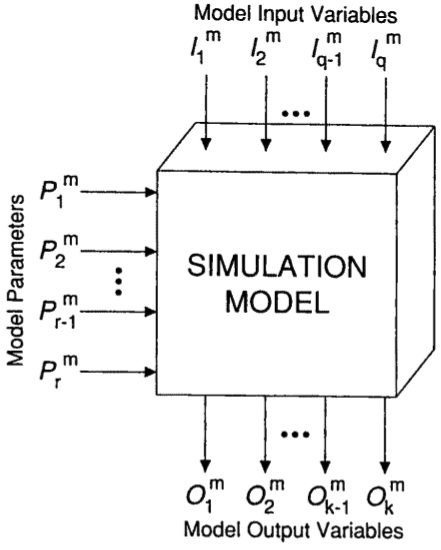
\includegraphics[width=.4\linewidth]{img/Balci1994a_Figure_Parametres.png}
	\caption{Les variables d'un modèle de simulation selon Balci \autocite[122]{balci_validation_1994-2}.\\
		\textit{Nota bene} : ce schéma est tronqué, ne présentant que la partie \og modèle de simulation\fg{} alors que celle-ci est mise en mirroir à une partie \og système\fg{} représentant l'empirique.}
	\label{fig:parametres-Balci} 
\end{figure}

Dans ce schéma et l'article associé, et bien qu'il n'en définisse nulle part explicitement le sens, Balci esquisse la composition d'un modèle de simulation.

\colorbox{pink}{\parbox{0.9\textwidth}{%
		\vskip5pt
		\leftskip5pt\rightskip5pt
		Décrire le schéma de Balci point par point. Faire un schéma pour Treuil, puis introduire les miens en les explicitant complètement.
		\vskip5pt
	}
}


\subsubsection{Paramètres, variables, indicateurs : un essai de définition}
\label{subsubsec:mes_definitions_params}

Nous considèrerons donc plutôt les paramètres comme le sous-ensemble des entrées, qui peuvent s'exprimer sous forme numérique (excluant donc de fait certaines entrée telles que les configurations spatiales initiales), et que l'on fera varier, aussi bien dans la calibration du modèle que pour l'exploration de scénarios.


\colorbox{pink}{\parbox{0.9\textwidth}{%
		\vskip5pt
		\leftskip5pt\rightskip5pt
		Faire un schéma avec organisation des variables/paramètres/entrées/sorties telles que proposée dans ma thèse.
		\vskip5pt
	}
}



\begin{figure}[!h]
	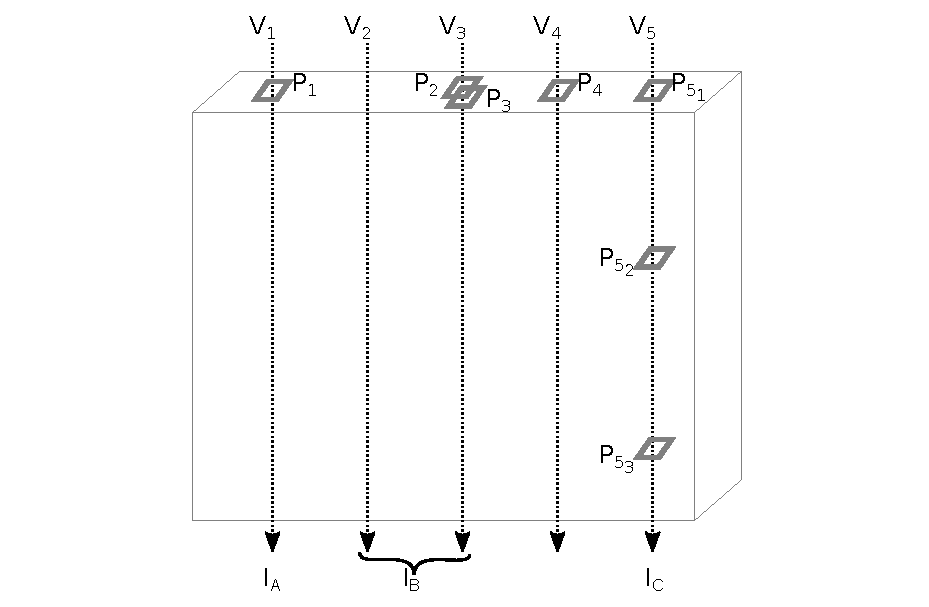
\includegraphics[width=\linewidth]{img/schemas_params_simple.pdf}
	\caption{Schématisation des définitions de variables (V), indicateurs de sortie (I) et paramètres (P).} 
	\label{fig:parametres-these-simple} 
\end{figure}

\colorbox{pink}{\parbox{0.9\textwidth}{%
		\vskip5pt
		\leftskip5pt\rightskip5pt
		Ne pas oublier de préciser différence entre paramètres et situation initiale. Ex. de situation initiale : des variables déjà allouées, par ex. pop des villes.
		Il n'y en a pas vraiment dans mon modèle pk tout est endogénéisé : pas de situation initiale, mais des paramètres qui définissent la création de celle-ci.
		\vskip5pt
	}
}

\begin{figure}[!h]
	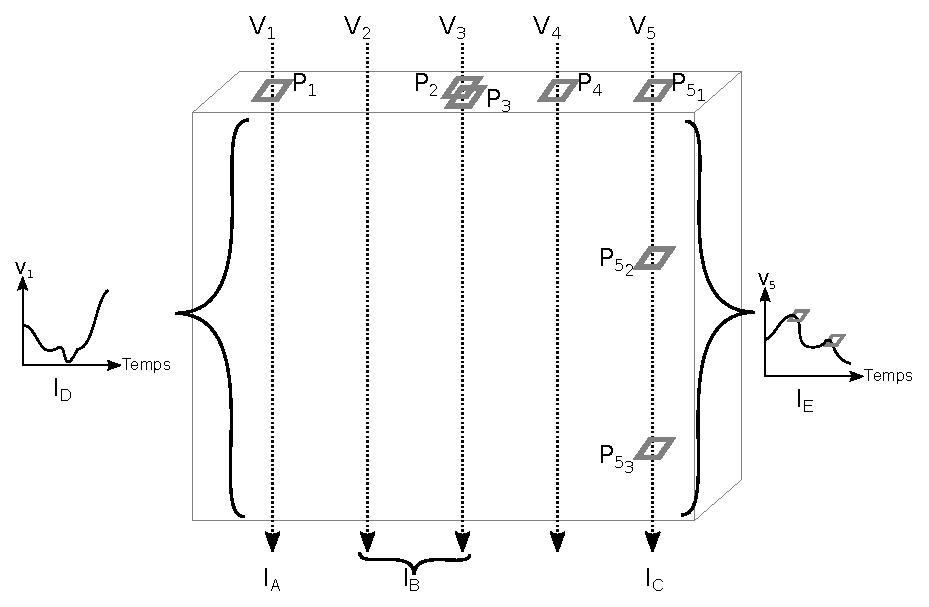
\includegraphics[width=\linewidth]{img/schemas_params_complet.pdf}
	\caption{Schématisation des définitions de variables (V), indicateurs de sortie (I) et paramètres (P) incorporant l'aspect temporel de certains indicateurs ($\text{I}_{\text{D}}$ et $\text{I}_{\text{E}}$).} 
	\label{fig:parametres-these-complet} 
\end{figure}

\newpage
\subsubsection{Paramètres et variables}

\begin{encadre}{Variables, entrées, paramètres\ldots}{termes-variables}
	Au sein des \textbf{variables}, constituées par l'ensemble des éléments d'un modèle ayant la capacité de changer, que ce soit au cours d'une simulation ou au travers de plusieurs expérimentations, nous distinguerons trois types spécifiques.
	\begin{description}[style=nextline]	
		\item[Entrées] Les \textbf{entrées} constituent l'ensemble des informations nécessaires à l'exécution d'un modèle en ce qu'elles en alimentent les mécanismes. Elles peuvent être constantes au cours d'une simulation (la date de fin d'exécution de notre modèle par exemple), ou évoluer de par l'action du modèle (le nombre d'églises paroissiale du modèle, qui est une entrée, et augmente tout au long de la simulation).
		
		\item[Paramètres] Certaines de ces entrées sont des \textbf{paramètres} : ce sont les entrées qui peuvent être mobilisées afin de modifier le comportement du modèle, et qui \og représentent ce que le simulateur peut perturber\fg{}\footnote{Pour reprendre les mots de Treuil et al. qu'ils appliquent aux entrées\autocite[8]{treuil_modelisation_2008}. }. Dans cet ouvrage, nous distinguerons plusieurs types de paramètres (\cref{enc:types-parametres}) selon leur ancrage dans l'empirique. Notons toutefois dès maintenant que le nombre de paramètres d'un modèle peut être bien supérieur au nombre de paramètres que l'on fera réellement varier dans les expérimentations.
		
		\item[Sorties] \hl{Les sorties d'un modèle représentent ce que l'on va observer après l'exécution du modèle afin d'observer son déroulement et aboutissement}.\footnote{Pas clair}.
		Ces sorties peuvent être très nombreuses, et concerner autant les variables individuelles (une liste des Foyers Paysans et de leur satisfaction au cours du temps par exemple) que des variables agrégées (Quartiles de satisfaction des foyers paysans par exemple), moins coûteuses en temps d'écriture ainsi qu'en espace de stockage. De la même manière que pour les paramètres, sur l'infinité potentielle de sorties d'un modèle, seules quelques-unes seront effectivement générées et enregistrées afin de minimiser les données produites à celles que le modélisateur compte explorer.
	\end{description}
\end{encadre}

\subsubsection{Différents types de paramètres}


Les paramètres sont donc un sous-ensemble des entrées d'un modèle qui ont vocation à varier dans les différentes exécutions de ce modèle. Pour autant, c'est un sous-ensemble assez divers, et tous les paramètres n'apportent pas les mêmes connaissances, que ce soit par leur valeur ou par la manière dont ils varient. Il convient donc d'identifier différents types de paramètres, non selon leur caractéristique propre (c'est-à-dire leurs propriétés, qui permettent de les différencier des sorties par exemple), mais selon leur usage et donc la manière dont on pourra les mobiliser. A ce titre, quand la littérature en sciences humaines et sociales\footnote{En physique ou en mathématiques par exemple, une telle distinction n'existe pas, la définition d'un paramètre prenant une considération plus simple d'élément rendu constant dans une exécution d'un modèle. \hl{pas clair, prendre une définition quelconque reprenant cette idée.}} distingue souvent (\hl{refs}) deux types de paramètres : les paramètres empiriques, dont la valeur a une correspondance directe dans le domaine empirique (on peut donc l'observer), et les paramètres techniques\footnote{Mathian et Tannier \autocite{mathian_formalisation_2015} utilisent le terme de paramètre mécanique pour définir ce type de paramètres. Nous trouvons l'usage du mot technique plus approprié, en ce qu'il se différencie plus de l'empirique sur le pan de l'usage qui en est fait. De plus, chaque paramètre, empirique, technique ou autre, a un impact sur les mécanismes du modèle, de par la définition que nous empruntons des paramètres \cref{enc:termes-variables}. Nous préférerons donc ce terme de \og technique\fg{} pour éviter les confusions.}, pour lesquels cette correspondance n'existe pas. Comme dans la plupart des typologies ayant trait à la catégorisation de valeurs numériques, de nombreux paramètres peuvent se trouver à l'interface de ces deux classes. Nous en proposons donc une troisième, que nous avons choisi de nommer \og paramètres commensurables\fg{}\footnote{
	La définition du dictionnaire \og Le Petit Robert\fg{} pour ce terme est celle-ci :  \og  Se dit d'une grandeur qui a, avec une autre grandeur, une commune mesure.\fg{}\autocite{robert_nouveau_1993}. \\Cf. aussi :			
	\og Les mondes n'apparaissent commensurables ou incommensurables qu'à ceux qui s'attachent aux mesures mesurées. Or, toutes les mesures, en science dure comme en science souple, sont aussi des mesures mesurantes et celles-là construisent une commensurabilité qui n'existait pas avant leur mise au point.\fg{}\autocite[153]{latour_nous_2013}},
qui nous semble à même caractériser des paramètres partiellement inscrits dans l'empirie, c'est-à-dire sans valeur empirique propre, mais permettant tout de même d'être mobilisés comme les paramètres empiriques, c'est-à-dire à même d'être comparés, que ce soit par les fluctuations de leurs propres valeurs ou en comparant des paramètres commensurables les uns avec les autres. Avec cette typologie des paramètres basées non sur la nature de ceux-ci mais sur leur utilisation dans un modèle, nous nous inscrivons dans une vision fonctionnaliste et donc très subjective, rappelant la définition d'un modèle de Minsky\footnote{\hl{Cf. sans doute le chapitre 1, à faire.}} \autocite{minsky_matter_1965}. Pour différents modélisateurs, un même paramètre pourra donc être considéré comme empirique ou commensurable, ou encore comme commensurable ou technique.
\colorbox{pink}{\parbox{0.9\textwidth}{%
		\vskip5pt
		\leftskip5pt\rightskip5pt
		Ne pas oublier de préciser que selon le point de vue du modélisateur, un paramètre peut passer de empirique à commensurable, ou de commensurable à technique (et vice-versa), mais pas \og franchir\fg{} toutes les catégories.
		\vskip5pt
	}
}


\begin{encadre}{Trois types de paramètres}{types-parametres}
	
	\colorbox{pink}{\parbox{0.9\textwidth}{%
			\vskip5pt
			\leftskip5pt\rightskip5pt
			Regarder s'il y a des enquêtes sur les seuils de satisfaction de Schelling dans la littérature.
			\vskip5pt
		}
	}
	
	\begin{description}
		\item[Paramètres empiriques] Les paramètres empiriques sont les paramètres qui peuvent être fixés à l'aide d'une ou de valeur(s) empiriquement connue(s), ou à défaut, dont la valeur se réfère à une quantité directement identifiable par une personne ayant des connaissances thématiques sur ce qui est modélisé.
		\begin{mdframed}[backgroundcolor=gray!10,footnoteinside=false]
			Dans le modèle de Schelling (\ref{desc:schelling}), le paramètre \fixref{\texttt{S}} est un paramètre empirique : la valeur qui lui est donnée peut être interprétée empiriquement, quand bien même il serait difficile d'obtenir, par exemple d'un enquêté, une valeur exacte à utiliser.
		\end{mdframed}
		\item[Paramètres techniques] Il s'agit des paramètres dont la valeur, ou même son ordre de grandeur, n'apportent aucune connaissance thématique au modélisateur. Ces paramètres ont pour raison d'être de permettre à d'autres types de paramètres de s'exprimer en valeurs compréhensibles et exploitables. Dès lors, leurs valeurs sont propres à chaque modèle formalisé, et une comparaison de ces valeurs entre les différents modèles n'apporte pas de connaissance.
		
		\begin{mdframed}[backgroundcolor=gray!10,footnoteinside=false]
			Dans le modèle gravitaire (\cref{desc:gravitaire}), $k$ est un paramètre technique : c'est un ratio qui varie afin d'ajuster l'ordre de grandeur des masses ($M_i$ et $M_j$) à celui des flux  échangés ($F_{ij}$). C'est une valeur d'ajustement, qui ne peut être comparée entre des modèles portant sur différents espaces et/ou thématiques\footnotemark.
		\end{mdframed}
		
		\item[Paramètres \og commensurable \fg{}]
		
		Cette catégorie, forgée dans le cadre de cet ouvrage, permet de représenter les paramètres qui ne sont pas fondamentalement issus de l'empirique mais qui peuvent toutefois être interprétés, que ce soit par rapport à une valeur canonique, définissant alors un repère, ou alors par rapport à d'autres valeurs de ce même paramètre, créant dès lors une échelle d'analyse. Outre la calibration d'un modèle, les valeurs de ces paramètres ont donc un intérêt propre et peuvent être analysées. pour elles-mêmes.
		
		\begin{mdframed}[backgroundcolor=gray!10,footnoteinside=false]
			Dans le modèle gravitaire (\cref{desc:gravitaire}), le frein de la distance (paramètre $\alpha$) peut être considéré comme un paramètre commensurable. Sa valeur ne renvoit ainsi à aucune dimension empirique, mais son usage répandu permet de comparer les valeurs qu'il peut prendre à des valeurs bien connues. Par exemple, on utilise fréquemment des valeurs de $\alpha$ comprises entre $1$ et $2$ pour exprimer la friction de la distance dans les navettes domicile-travail. Une valeur inférieure à $1$ peut donc être interprétée comme laissant une part plus faible à la distance, par exemple dans le cas de déplacements de loisirs. A contrario, un paramètre $\alpha$ supérieur à $2$ montrera une plus forte friction de la distance, par exemple dans les choix d'une école élémentaire à proximité du foyer d'un ménage.
		\end{mdframed}
	\end{description}
	\footnotetext{Dans le cas où $\alpha$ vaut $0$, ce paramètre peut être vu comme commensurable dans la mesure où il devient alors la part de la masse qui devient un flux.}
\end{encadre}


\subsubsection{Comment choisir les valeurs de paramètres ?}

\hl{Ici, faire un court paragraphe de transition pour présenter rapidement l'approche générale du paramétrage : peut-être redondant avec ce qui suit, en particulier dans les présentations des paramètrages du modèle gravitaire et de Schelling.}

\subsection{Le paramétrage, un processus d'amélioration du modèle.}

Le paramétrage d'un modèle est souvent réduit à l'un de ses aspects, le \og calibrage \fg, étape finale de la construction d'un modèle qui cherchera à reproduire autant que possible des données empirique en faisant varier les valeurs des paramètres jusqu'à ce qu'une combinaison de celles-ci soit satisfaisante.

De nombreux auteurs ont montré que le paramétrage d'un modèle ne pouvait se réduire à cette étape, chacun employant des termes différents pour désigner le processus de paramétrage.

%%%% Pas adapté  %%%%
Gilbert et Troitzsch \autocite{gilbert_simulation_2005} restent très flous en utilisant les termes de \textit{checking} et de \textit{debugging}, qu'ils inscrivent dans une démarche plus large de \textit{verification} correspondant à la \hl{validation interne}\footnote{\hl{Définir !}}.
Osman Balci \autocite{balci_validation_1994-2} crée et emploie l'acronyme \og \textit{VV\&T}\fg{}\footnote{\textit{Validation, Verification and Testing}}, à portée plus large puisqu'il s'applique à chacune des étapes de la modélisation
%%%%  %%%%

Le plus souvent (\fixref{ref Seb, Clem...}), une fois le modèle construit, le modélisateur s'attache à son \og calibrage\fg{}, en cherchant pour chaque paramètre la ou les valeurs qui permettront au modèle de s'approcher des données empiriques devant être reproduites.
Cette étape, que l'on nomme généralement calibration, peut se faire de manière manuelle, par approximations successives (\fixref{C. Cottineau et/ou S. Rey, d'après Hermann}), par semi-automatisme, \change{Lena : trouver d'autres exemples plus classiques et lointains}{exemple en effectuant des analyses de sensibilité} (\fixref{C. Schmitt, J. Hirtzel}), ou encore de manière entièrement automatique (\fixref{C. Schmitt, S. Rey, C. Cottineau avec PSE}).
L'approche souvent défendue, notamment dans les travaux les plus récents (\fixref{Rimbault?}), voudrait que cette étape soit obligatoire pour toute modélisation, permettant par une exploration systématique de comprendre l'entièreté du comportement d'un modèle, et d'en faire dès lors un outil complètement maitrisé \change{Lena: expliciter}{rendant possible l'établissement d'une loi}.

Dans notre travail, nous souhaitons revenir sur cette approche de la modélisation, ancrant le paramétrage comme étape ultime de la construction d'un modèle, en particulier en ce que nous considérons que cette pratique de recherches de \change{Lena : penser à bien l'introduire avant.}{valeurs optimales} est un exercice qui devrait s'effectuer tout au long de la construction du modèle, de manière plus itérative que conclusive.


\subsection{Qu'est-ce que le(s) paramétrage(s) ?}

\subsubsection{Définition}

\change{J'aime bien cette définition, c'est la seule à avoir le sens que j'entends dans paramétrage/paramétrer. Et elle introduit une logique d'optimalité.}{Paramétrer (informatique): \og Programmer (un appareil complexe), en définissant les paramètres assurant son fonctionnement optimal. Ex. \textit{Paramétrer une imprimante}\fg{}\autocite{robert_nouveau_1993}.}

Le terme recouvre deux sens différents, dont la distinction peut se faire selon qu'on l'utilise pour définir un processus ou pour caractériser une configuration.
Ici, nous emploierons plutôt le premier cas, définissant dès lors le paramétrage comme le processus, manuel ou automatique, visant à constituer cette configuration de paramètres.
Dans ce deuxième cas, le paramétrage désigne un ensemble de valeurs de paramètres, par exemple quand on mentionne un paramétrage par défaut, ou un paramétrage optimal.
Pour ne pas risquer de contre-sens, nous préférerons le terme de configuration de paramètres.

On tend à distinguer le paramétrage -- passage obligé ne nécessitant pas d'être évoqué -- de la calibration, processus systématique qui inscrirait le modèle comme un outil scientifique et incontestable.
Nous choisissons ici de confondre ces approches, non pas en considérant le paramétrage comme un outil d'évaluation du modèle, mais comme une composante inhérente à la construction d'un modèle, quelque soient les formes et les temporalités que le paramétrage adopte.
Le paramétrage est en effet une pratique utile dans la construction du modèle, car les résultats auxquels il aboutit, c'est-à-dire les valeurs de paramètres qui semblent mieux adaptés, renseignent aussi bien sur les biais des mécanismes adoptés que sur leur efficacité réelle.
Par exemple, quand, après avoir ajouté un mécanisme, on se rend compte que des variations dans les valeurs de paramètres ne changent pas réellement les sorties du modèle, cela peut être l'occasion de repenser le mécanisme dans son ensemble, ou plus souvent, la manière dont le paramètre est mobilisé dans ce mécanisme. On retrouve cette logique dans l'exploration par Clara Schmitt du modèle SimpopLocal \autocite{schmitt_modelisation_2014-1}, qui a permis de réaliser que la variation de l'un des paramètres ($InnovationLife$) n'avait que peu d'impact sur les sorties du modèle, tout en rendant sa calibration plus complexe et instable :
\begin{quote}
	Au dessous du seuil des 150 pas de simulation pour le paramétrage de InnovationLife, le calibrage du modèle est très difficile voire impossible. Au dessus de ce seuil, le mécanisme associé au paramètre InnovationLife n’a plus d’effet sur le calibrage du modèle. Dans un soucis de parcimonie du nombre et de la complexité des mécanismes simulés dans le modèle SimpopLocal, il est justifiable de retirer du modèle ce mécanisme qui n’est pas nécessaire à la simulation de la dynamique de croissance recherchée.\\
	\mbox{}~ \hfill \autocite[224]{schmitt_modelisation_2014-1}
\end{quote}

\paragraph{}Afin d'illustrer ces propos, on peut s'appuyer sur des modèles bien connus de la littérature, issus de deux champs disciplinaires différents.

\subsubsection{Illustration : le modèle gravitaire.\label{desc:gravitaire}}

\paragraph{Description}	Ce modèle statistique\footnote{Pour une description plus complète, se référer à l'ouvrage de Pumain et Saint-Julien \autocite{pumain_les_2001}.}, dans la formulation qu'en a faite Stewart \autocite{stewart_demographic_1948}, vise à prédire des flux (démographiques, marchands etc.) potentiels entre des lieux à partir d'une analogie avec la loi physique de la gravitation. Dans le formalisme le plus simple, \og sans contrainte\fg{} \autocite{pumain_les_2001}, on peut l'exprimer ainsi :
$$
F_{ij} = \frac{k \times M_{i} \times M_{j}}{d_{ij}{}^\alpha}
$$
Ce modèle présente trois valeurs empiriques ($M_i$, $M_j$ et $d_{ij}$) et deux paramètres ($k$ et $\alpha$). $k$ est un paramètre technique (\cref{enc:types-parametres}), puisque bien que basée sur l'empirique, sa valeur -- et les fluctuations de celle-ci -- ne donne aucune information sur le système étudié. $\alpha$ est un paramètre commensurable pour les raisons explicités dans l'\cref{enc:types-parametres}.

À partir des valeurs empiriques $M_i$ et $M_j$ qui caractérisent les masses (populations, ou stocks de  marchandise par exemple) des lieux $i$ et $j$, et de la distance qui les sépare $d_{ij}$, on peut ainsi prédire $F_{ij}$, le flux entre ces lieux.

\paragraph{Objectif} Afin que ce modèle donne des ordres de grandeur réalistes quand aux quantités échangées, il faut le paramétrer en définissant une valeur de $k$, permettant dès lors d'obtenir un rapport entre les masses d'origine et les quantités échangées.
La valeur de ce paramètre est conditionnée par celle de $\alpha$, que l'on nomme fréquemment \og frein de la distance\fg{}, en ce qu'il permet de quantifier l'impact qu'aura un éloignement plus ou moins important sur la quantité de flux échangés.

\paragraph{Paramétrage} Pour \og ajuster\fg{}\footnote{C'est le terme employé par \autocite{pumain_les_2001}, que l'on peut ici retenir comme équivalent de paramétrer. François Durand-Dastès  \autocite[298]{durand1995modeles} utilise pour sa part le terme de calibration à propos du même modèle.} le modèle, il faut donc en réaliser le paramétrage en s'appuyant sur les éléments connus de l'équation (les valeurs empiriques).
$\alpha$ et $k$ étant liés dans l'équation, la valeur de chacun de ces paramètres dépend de celle choisie pour l'autre, et un changement dans l'un des paramètres entraînera la nécessité de modifier l'autre.

Le paramétrage le plus simple consiste à réaliser une régression linéaire sur les logarithmes décimaux des distances et des flux observés, $k$ prenant alors la valeur du logarithme de l'ordonnée à l'origine et $\alpha$ celle du coefficient directeur de la courbe.	
Le modèle est alors calibré (voir \cref{enc:termes-calibration}), mais si l'on souhaite donner une valeur spécifique à l'un des paramètres, par exemple pour utiliser une valeur classique de 2 au frein de la distance ($\alpha$) \autocite{pumain_modegravitaire_2004}, il faudra alors le re-soumettre à paramétrage pour adapter $k$. De même si l'on modifie les lieux et/ou les masses sur lesquels il s'applique.


\subsubsection{Illustration : le modèle de ségrégation de Schelling.\label{desc:schelling}}

\paragraph{Description}Le modèle de Schelling\footnote{Une description plus poussée accompagnée d'une description de l'exploration du modèle peut être lue dans \autocite{daude_comparaison_2006}} est un modèle de simulation décrit par Thomas Schelling \autocite{schelling_dynamic_1971} qui vise à montrer comment un espace peut passer d'un état intégré à un état ségrégé ethniquement à travers une succession de comportements individuels de mobilité résidentielle. Il montre en particulier qu'on peut parvenir à un état ségrégé même quand les comportements individuels sont majoritairement tolérants.

L'espace du modèle est défini comme une grille carrée composée de $N$\footnote{Nous reprenons ici la notation $M(N, d, n, S)$ proposée par \autocite[433]{daude_comparaison_2006} en n'explicitant toutefois pas le paramètre $n$ décrivant le type de voisinage (4 ou 8) utilisé.} cellules.
Au début de la simulation, des agents de deux types, en proportions similaires, sont distribués aléatoirement dans l'espace du modèle. Chaque agent occupe une cellule, et le nombre total de cellules occupées (et donc d'agents) dépend d'un paramètre de densité $d$ qui représente la part (entre $0\%$ et $100\%$) du nombre de cellule qui sera occupé\footnote{Il y a donc $N \times d$ agents, et donc $\frac{N \times d}{2}$ agents de chaque type.}.
Chaque agent est défini par une satisfaction. Celle-ci correspond à la part de cellules voisines occupées par des agents \og étrangers\fg{}, c'est-à-dire d'un autre type : plus le voisinage contient d'étrangers, moins l'agent est satisfait.
Si cette satisfaction est inférieure à un paramètre de tolérance $S$, l'agent est considéré comme insatisfait et se déplace aléatoirement dans une cellule non occupée.
A terme, Schelling montre que même en considérant des valeurs de $S$ assez élevées, c'est-à-dire un comportement plutôt tolérant, la succession de choix individuels entraîne la mise en place d'une distribution spatiale très ségrégée.
On considère que le modèle a convergé quand l'ensemble des agents sont satisfaits, ce que ne permettent pas toutes les combinaisons de valeurs de paramètres.

Dans ce modèle, on peut donc dénoter trois paramètres, $N$, $d$ et $S$. Les deux premier sont des paramètres techniques (\cref{enc:types-parametres}), en ce que, purement théoriques, ils ne se réfèrent à aucune quantité empirique, ni ne peuvent être utilisés afin de se référer à un ordre de grandeur connu qui en ferait des paramètres commensurables. $S$ est un paramètre empirique. Bien que le modèle soit théorique, ce paramètre se réfère toutefois à une comportement ayant un sens empirique fort.

\paragraph{Objectif} Le paramétrage de ce modèle consiste à fixer un $N$ constant et à faire varier $d$ et $S$ afin d'en trouver des valeurs permettant la convergence vers une situation stable. Quand $d$ est très faible ($30\%$ dans l'exemple de \autocite{daude_comparaison_2006}), quelles que soient les valeurs de $S$, le modèle converge rapidement : quand l'espace du modèle dispose d'une faible densité d'agents, il est facile pour ceux-là de créer des agrégats homogènes distants d'agrégats de l'autre type d'agents. Quand $d$ est plus important ($\geq66\%$), l'espace disponible étant limité, toutes les valeurs de $S$ ne permettent pas la convergence du modèle. Le paramétrage du modèle aura donc pour objectif de trouver la valeur maximale possible -- pour un $N$ et un $d$ donné -- que peut prendre le paramètre de tolérance $S$ tout en laissant le modèle converger.

\paragraph{Paramétrage}Contrairement au modèle gravitaire, le modèle de Schelling est stochastique : les agents se déplacent aléatoirement quand non satisfaits. Dès lors, deux exécutions du modèle avec le même jeu de paramètres n’entraîneront pas forcément la même configuration spatiale. Qui plus est, pour certains jeux de paramètres, seules certaines exécutions convergeront. Le paramétrage de ce modèle ressemble donc à celui qui est réalisé pour le modèle SimFeodal. La manière \og traditionnelle\fg{}\footnote{C'est-à-dire manuelle, au contraire de méthodes automatiques plus rigoureuses et récentes.} consiste à fixer un $d$, puis à essayer d'augmenter le $S$ tant que le modèle converge. Si le modèle converge pour tout $S$, on augmente la valeur de $d$ et on recommence à chercher la valeur maximale possible pour $S$. De part la nature stochastique du modèle, chaque jeu de paramètres doit être simulé plusieurs fois, le nombre de ces réplications dépendant de la part d'aléa dans le comportement du modèle.
Un modèle de Schelling calibré, c'est-à-dire dont le paramétrage est achevé,
donnera pour un $N$ fixé les valeurs maximales de $d$ et de $S$ atteignables.

\paragraph{}A travers ces deux exemples ayant traits à des méthodes différentes, on retrouve deux approches de paramétrage que l'on souhaite ici voire confondues : dans le premier cas, le paramétrage du modèle gravitaire tend à sa calibration, à la recherche d'une solution optimale, c'est-à-dire meilleure que toute autre. Pour un phénomène donné (un jeu de données précis par exemple) et un formalisme donné (l'expression la plus simple du modèle, ici sans contrainte), seule un couple de paramètres $\alpha$ et $k$ permet ainsi d'obtenir des flux modélisés proches des flux observés.
Dans le cas du modèle de Schelling, il n'y a pas de recherche d'optimum : le paramétrage permet de comprendre le modèle en en définissant les limites en matière de convergence. Une configuration de paramètres $S$ et $d$ ne sera pas meilleure qu'une autre, mais pour un $S$ donné, on saura quel est la valeur maximale de $d$ permettant cette convergence (et réciproquement).

\subsubsection{Paramétrer un ou des modèles ?}

\change{Lena : trop endogame, prendre exemples modèles modulaires dans JASSS}{\fixref{Cottineau, Reuillon et Rey} ont montré qu'on construisait plus souvent des familles de modèles que des modèles uniques.}
Ces auteurs plaident pour une construction modulaire de modèles, chacun des mécanismes et complexifications devant être autonomes afin de pouvoir les assembler en autant de combinaisons que nécessaire à une exploration d'ensemble de leurs interactions.

Nous reprendrons de leur discours une vision moins ambitieuse, en considérant (\changec{ref Rey}{à chercher il en parlait à sa soutenance je crois}) simplement qu'en fait d'un modèle, la modélisation passe par plusieurs modèles, ayant chacun différentes implémentations d'un mécanisme conceptuellement identique et chacun se devant dès lors d'être adapté par un paramétrage dédié.

Pour illustrer ce propos, on peut prendre l'exemple d'une modification qui a eu lieu sur notre modèle au cours de son développement. On considérait jusque là que pour prendre en compte la population rurale (hors Tours donc), $1000$ foyers paysans donnaient une bonne idée de la situation en 800 pour l'espace considéré.
Lors d'une réunion, les thématiciens se sont rendus compte que ce nombre sous-estimait très largement la population réelle, et qu'il valait mieux passer ce paramètre à $4000$ foyers paysans.
Les autres paramètres, fixés en bonne partie empiriquement, n'avaient visiblement aucune raison d'évoluer du fait de ce changement. Les mécanismes  et effets de seuil étaient en effet conçus de manière à être relatifs aux masses manipulées, et le changement attendu était une augmentation linéaire des indicateurs de sortie.

\begin{figure}[H]
	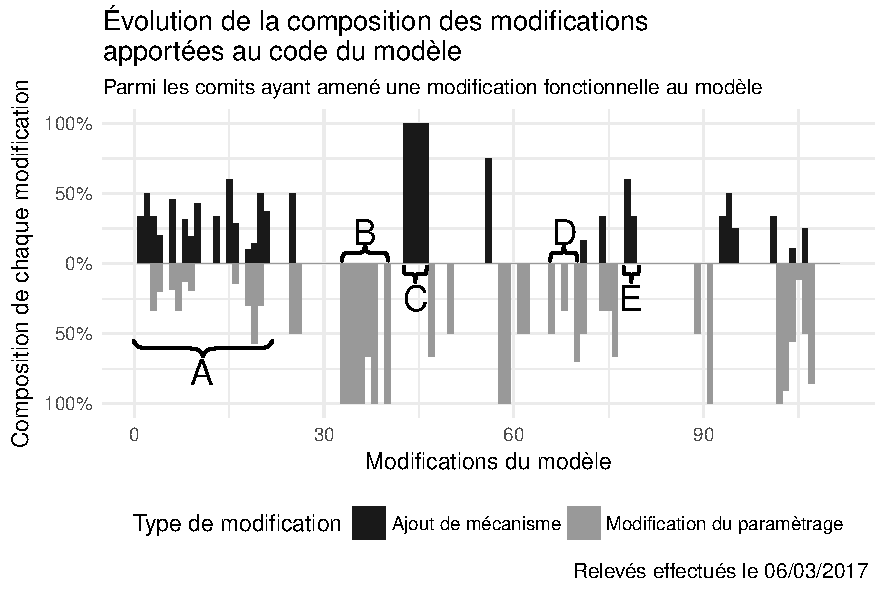
\includegraphics[width = \linewidth]{img/plotComits.pdf}
	\caption{Temporalité du paramétrage du modèle.\\
		Chaque \og enregistrement\fg{} (\textit{comit}) correspond à une version modifiée et sauvegardée du modèle, contenant un ou plusieurs changements. On a ici rapporté le nombre de changements de chaque type (modification de mécanisme ou de valeur de paramètre) au nombre total de changements de chaque \textit{comit} afin de figurer l'évolution des types de modification au cours de la construction du modèle.}
	\label{fig:comits-periodes}
\end{figure}

Dans les faits, cette légère modification a entraîné une obligation de repenser la quasi-totalité des autres paramètres et d'ajuster une bonne part des règles. 
La concentration des foyers paysans était en effet bien trop rapide avec autant d'individus, et le modèle convergeait en quelques pas de temps vers une configuration presque statique et très concentrée.
Tous les mécanismes de régulation de ce comportement étaient dès lors rendus ineptes, et il a fallu changer en profondeur la manière dont chaque paramètre et mécanisme interagissait avec les autres.
\change{Lena : Là on ne suit pas, mais ce sera explicité dans le chap. 2}{C'est un changement majeur, que l'on peut constater dans la figure~\ref{fig:comits-periodes} (1ère modification de la période B), ayant donc entraîné des adaptations de tous les plans du modèle (paramètres en B, mécanismes en C).}
La première version avait été paramétré aussi correctement que possible, mais ce paramétrage était entièrement à refaire avec la nouvelle version (modifications de la période B, \cref{fig:comits-periodes}).
\change{Lena : à discuter plus profondément}{On pourrait dès lors différencier le modèle pré-existant et celui qui a suivi ce changement, et les considérer comme deux modèles puisque réagissant de manière extrêmement différente.}

\change{Lena: Pas clair et pas assez logique}{Cet exemple renforce le caractère nécessaire du paramétrage, et qui plus est, de la continuité de cette étape, qui ne peut être pensée que comme une calibration finale d'un modèle abouti, auquel on ne peut en fait parvenir que par des paramétrages réguliers de modèles successifs moins aboutis.}

\subsubsection{Désambiguïsation}

De nombreux termes sont utilisés dans la littérature, souvent sans réelle distinction, pour désigner cette opération qui consister à choisir un jeu de paramètres pour un modèle. Pêle-mêle, on y retrouve le paramétrage, la validation, l'évaluation ou encore la calibration. Nous définissons dans l'\cref{enc:termes-calibration} le sens donné à chacun de ces termes dans le cadre de ce manuscrit.
\bigskip

\begin{encadre}{Calibration, évaluation, validation\ldots}{termes-calibration}
	\begin{description}[style=nextline]	
		\item[Calibration] On réserve souvent, et nous nous y tiendrons, ce terme à la dernière étape dans l'aboutissement d'un modèle.
		Une fois les mécanismes fixés et des objectifs définis, on peut procéder à la calibration, c'est-à-dire à une exploration de l'espace des paramètres ayant pour but de stabiliser les paramètres afin de se rapprocher autant que possible de ces objectifs.
		Cette étape, quelques soient les moyens employés, s'approche de la résolution utilisée dans le cadre de systèmes d'équations.
		Le contexte des systèmes complexes, et donc d'une non-linéarité des effets des paramètres, rend toutefois difficile l'obtention d'une unique configuration de \hl{paramètres optimale}\footnote{Lena : il faut partir d'une def plus basique en intro}, et la calibration aboutit donc souvent à un ensemble de configurations possibles, constituant par exemple un optimum de Pareto (\fixref{Trouver ref}).
		
		\item[Évaluation] On emploie majoritairement ce mot pour décrire les méthodes permettant de comprendre le comportement du modèle et sa réaction aux différents paramètres.
		Là où la calibration cherche une configuration de paramètres optimale, l'évaluation tend surtout à caractériser la stabilité du modèle face à l'aléa ou a des configurations exceptionnelles.
		On vise ainsi à s'assurer que le modèle reproduise \hl{les faits stylisés}\footnote{Lena : pas introduits avant} voulus quelque soient son réglage, ou au moins à quantifier les intervalles de paramètres qui y satisfont.
		
		\item[Validation] La validation (refs Seb) tire son origine de sciences plus nomothétiques, et correspond donc à la démonstration qu'un modèle reproduit correctement ce qu'il représente. Au delà de l'évaluation, le terme amène une logique de preuve formelle que le modèle réagit bien ainsi et pas autrement quelque soient les conditions d'exécution. Cette démonstration formelle peut être effectuée sur des modèles à faible nombre de paramètres et mécanismes, mais le terme n'est jamais (à vérifier) employé dès lors que les modèles se complexifient.\footnote{Lena : cf. JASSS : Faire un rappel du sens classique, par ex. en stats.}
	\end{description}
\end{encadre}


\subsection{Comment paramétrer ?}

\subsubsection{Visual validation}

(Trouver ref dans thèse Clémentine, sans doute Hermann encore)

\subsubsection{Indicateurs}

\subsubsection{L'importance de la réplication}
